\def\tu{\vec\theta_{\uparrow}}
\def\td{\vec\theta_{\downarrow}}

\subsection{Linear Regression}

% TODO: Cite sources:
% - https://www.kaggle.com/c/house-prices-advanced-regression-techniques/data


% TODO: Sprinkle in actual examples from the data. Right now the explanation is highly theoretical, which is far from what we are trying to do (even though the concepts are purely theoretical...)

% TODO: Explain this better. It sounds robotic and unintuitive. This shit needs
% to be a STORY
The main focus of this section is predicting a real number when given a set of
other numbers, or using pre-recorded inputs and outputs to generate new outputs
for any input we may need. In a linear sense, we are finding a continuous
function that takes in one number and spits out another using previously
gathered data. So the question is, how do we form this function?


Let's look at the scatterplot in Figure \ref{fig:hp}, which shows a bit of
housing data from Ames, Iowa. When observing it, our goal is to create a model
that will take a plot area and give us a house price that best fits the examples
recorded. So we start by asking, what kind of representation of data best aligns
with what we are asking? How can we find patterns in this data to predict what
price might be associated to a specified plot area? How can we do this
autonomously?

\begin{figure}[t!]
\centering
    \begin{tikzpicture}
        \selectcolormodel{gray}
        \begin{axis}[
                title = {HOUSE PRICES AND PLOT AREAS},  % whatever name you want
                xlabel = {Plot Area in 1,000 ft$^2$},
                ylabel = {House Price in \$100,000},
            ]
            \addplot[
                only marks,
                domain={4:18}
                ] table[col sep=comma]{linreg_houseprice.csv};
            \addplot[
            		gray,
            		thick,
            		dashed,
            		domain={4:18}
            ]{0.5 + 0.2*x};
            \addplot[
            		gray,
            		thick,
            		dotted,
            		domain={4:18}
            ]{0.1*x};
        \end{axis}
    \end{tikzpicture}
    \caption{List of plot areas and selling prices for houses in Ames, Iowa.
    Looking at these kind of plots, we can try to find correlations in the data
    that help us predict what future houses may cost in that market. The dashed line is our hypothesis with weights $\theta_{\uparrow}$ and the dotted line is our hypothesis with weights $\theta_{\downarrow}$.}
    \label{fig:hp}
\end{figure}

First, we can identify that there is a positive correlation when comparing each
plot area with its corresponding price, showing us that as plot area increases,
so does the house price. There are some outliers for this case, but generally
this trend is consistent. Additionally, we can take note that there is some
base price for every house in the area. Intuitively, we can
observe this by the fact that the goal of selling a house is to make money, so
assuming the smallest house you could buy is around 1,000 ft$^2$, we would
never see such a house costing \$0. As such, we should be able to draw a
straight line through the data from some offset such that we get fairly close
to all of the recorded examples.

This relationship is the basis for any linear function of the form $y=b + ax$
with the slope coefficient $a$ describing the correlation between housing
price/plot area and the offset or bias $b$ describing the overall starting price for
houses in Ames. We prescribe these coefficients to the vector of prices $\vec\theta
= \begin{pmatrix}\theta_0 \\ \theta_1\end{pmatrix}$ such that the base price is
$b = \theta_0$ and the price per ft$^2$ of plot area is $a=\theta_1$. This
coefficient vector is known as the \emph{weight vector} since we adjust the
values in $\vec\theta$ until we find coefficients that best fit the data. In
context, this linear function will predict the ideal price of any house in
Ames after learning from the experiences we feed it.

Let $X$ be the training set, i.e. the set containing all of the
recorded plot areas. Let $X^{(i)}$ be the plot area for the $i$th feature in
$X$. From what we've discussed about slope, the equation
\begin{equation}
    hypothesis_{\vec\theta}(X^{(i)}) = \theta_0 + \theta_1X^{(i)}
\end{equation}
should hypothetically give us the correct price for $X^{(i)}$.

Now that we have a method of predicting values, it is helpful to see how different choices of $\vec\theta$ interact with our hypothesis. Let us consider two such choices:
\begin{equation*}
	\vec\theta_{\uparrow} = \begin{pmatrix}50000 \\ 200\end{pmatrix} \quad 	\vec\theta_{\downarrow} = \begin{pmatrix}0 \\ 100\end{pmatrix}
\end{equation*}
. The first choice $\vec\theta_{\uparrow}$ has a base price of \$50,000 and increases by \$200 per ft$^2$ of plot area. The second choice $\vec\theta_{\downarrow}$ has a base at \$0 and increases by \$100. A meaningful question to then ask is: \emph{how well does our hypothesis predict values with these weights?}

For the first feature in our dataset with a plot area of 8,450 ft$^2$ we note the original price is \$208,500. When using weights $\vec\theta_{\uparrow}$ we will get the hypothetical price \$219,000 after calculation. Seems somewhat accurate, right? This price only overestimated the original by \$10,500 which is not terrible, specifically when compared to our hypothetical price  with weights $\vec\theta_{\downarrow}$, which gives us \$84,500 and underestimates the data by -\$124,000.

This measurement, the distance between our prediction and the recorded result, is defined as the \emph{loss} of our hypothesis. For the previous paragraph, we defined the loss as:
\begin{equation*}
	loss_{\vec\theta}(X^{(i)}) = hypothesis_{\vec\theta}(X^{(i)})-y^{(i)}
\end{equation*}
. There is an issue in this definition however, that being an inconsistent measurement between positive and negative values. Underestimations in the hypothesis, as we saw in $loss_{\vec\theta_{\downarrow}}(8450)$, result in a negative loss, which we can almost consider as a gain. This is flawed thinking since this is still an inaccuracy, and so should still be considered a loss. Considering this, we need a more consistant estimate for both overestimations and underestimations. The most apparent way of doing this would be taking the absolute value, making our loss function
\begin{subequations}
\begin{align}
	loss_{\vec\theta}(X^{(i)}) = |hypothesis_{\vec\theta}(X^{(i)}) - y^{(i)}| \\
	\intertext{. This is a completely viable option. Another way of achieving this is by squaring the loss }
	loss_{\vec\theta}(X^{(i)}) = (hypothesis_{\vec\theta}(X^{(i)}) - y^{(i)})^2
\end{align}
\end{subequations}
. Each of these have their own situational benefits discussed further in \placeholder, however we will suffice to square the loss for now.

Now let's get back to the original question: how well does our hypothesis predict values with these weights? Given what we have put together, it would make sense to say our hypothesis performs well when our weights have a low average loss across the data set since this would mean our average distance between every prediction and recorded value is low. This measurement, the effectiveness of our hypothesis using $\vec\theta$ across an entire data set, is called the \emph{cost} of $\vec\theta$. We then define the cost function as
\begin{subequations}
    \begin{align}
        cost(\vec\theta) =\underset {1\leq i\leq m}{average}(loss_{\vec\theta}(X^{(i)}, y^{(i)})) \\
    \intertext{or equivelently}
        cost(\vec\theta) = \frac{1}{m}\sum_{i=1}^m (\theta_0 + \theta_1X^{(i)} -
        y^{(i)})^2
    \end{align}
\end{subequations}
.

For our two choices of $\vec\theta$, we then have the costs
\begin{equation*}
	cost(\vec\theta_{\uparrow})= \$99,540.98 \quad \text{and} \quad cost(\vec\theta_{\downarrow}) = \$103,400.92
\end{equation*}
. Our cost for $\tu$ is lower than that of $\td$, meaning that $\tu$ generally predicts values closer to our data set than $\td$. Still, our lowest cost at the moment is \$99,540.98, meaning on average our hypothesis is off from our actual data by almost \$100k. We can do better than this.

Now that we have a method of evaluating our hypothesis's performance with weights $\vec\theta$, the next question is: what are values of $\vec\theta$ that minimize this cost?

We are looking for
a base price and price per ft$^2$ that matches the data enough such that the
hypothesized price would be reasonably close to the recorded price. What we're
essentially looking for are \emph{the coordinates of a point in the cost
function's domain that correspond to the lowest lowest possible value for the
cost}. To do this, let's consider the shape of the cost function.

The loss function expands out to be a second degree polynomial in two
dimensions, and we can identify each of the leading terms to be $\theta_0^2$ and
$\theta_1^2$. This is unaffected by the summation in the cost function, so it
has the same form. We visualize what this would look like in
Figure
\ref{fig:cost}. From there, we can see the inputs $\vec\theta$ and ouptuts of
$cost(\vec\theta)$ form an \emph{elliptical paraboloid}.

\begin{figure}[t!]
    \centering
    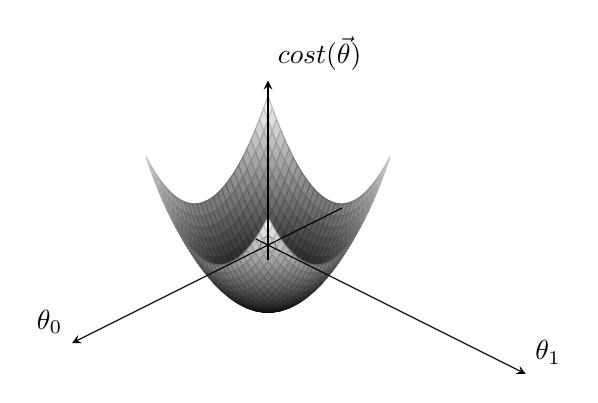
\begin{tikzpicture}[
        declare function = {
            Z(\x, \y) = ((\x-8)^2 + (\y-8)^2)/8;
        }
    ]
        \begin{axis}[
            view = {135}{30},
            colormap/blackwhite,
            axis equal,
            axis lines = center,
            axis on top,
            ticks = none,
            set layers = default
            xmin = 0, ymin = 0, zmin = 0,
            xlabel=$\theta_0$, ylabel={$\theta_1$}, zlabel={$cost(\vec\theta)$},
            xlabel style={anchor=south east},
            ylabel style={anchor=south west},
            zlabel style={anchor=south west},
            enlargelimits,
            tick align=inside,
            domain=0:16,
            y domain = 0:16,
            samples=30,
            z buffer=sort,
            minor tick=1,
            ]
            \addplot3 [surf] {Z(x, y)};
        \end{axis}
    \end{tikzpicture}
    \caption{The elliptical paraboloid formed by our weights $\vec\theta$ and $cost(\vec\theta)$.}
    \label{fig:cost}
\end{figure}


The coordinates we are looking for are then the exact point where this
paraboloid bottoms out since this is by definition the minimum of the cost function. We can obtain
this point by noting the graph has an \emph{inflection point} at the point $P =
(\theta_x, \theta_y)$ where we go from descending the paraboloid's curve to
ascending it. That is, if we were to take points $P_1$, $P_2$, $P_3$, and $P_4$
with $P_1 < P_2 < P < P_3 < P_4$ then $cost(P_2) - cost(P_1)$ would be negative
while $cost(P_4) - cost(P_3)$ would be positive. As we approach $P$ from either
side of the inflection, we expect to see the net change being
reduced to infinitely small amounts. This makes sense since at
$P$ we are neither descending or ascending and as we move closer to it we see
the amount change reflecting this. This is by definition when the gradient of
the cost function is 0: $\nabla cost(\vec\theta) = \vec{0}$.

% TODO: Site source https://stanford.edu/~rezab/classes/cme323/S16/notes/Lecture03/cme323_lec3.pdf
Solving for this gradient is, however, computationally infeasible. As we will
see later on, the growth of this type of function is much too large for many
modern computers to handle efficiently, especially as we begin adding more
components to our features. Even for this simple example, we end up attempting
to find solutions for a linear system of the form $A\vec\theta = B$, and so we could find these weights
by computing $\vec\theta =A^{-1}B$. This has a lower computational bound of
$O(n^{2.375})$ when using a variant of \emph{Strassen's algorithm} discovered by
Virginia Williams [Source]. $n$ in this case is the number of weights in
$\vec\theta$. However, the algorithm tends to only be advantageous over the naive
version of matrix multiplication when a specific RAM model (PRAM, for more see
[source]) is used and when $n \geq 1,000$. Otherwise, the traditional form of
matrix multiplication is nearly as effective. This puts us at a lower bound of
$O(n^3)$, which is highly inefficient when dealing with models of any caliber.

Because finding exact solutions is infeasible, we instead seek to approximate
these values as closely as we can. So how do we go from having unknown values of
$\vec\theta$ to precise values that approximate the dataset? The general idea is
that we want to pick a point in the domain and move this point along the direction of the curves until we reach the global minimum, almost as if we are trying to slide down the curve. We have to start
somewhere, and considering the parabolic shape in Figure \ref{fig:cost} contains a
global minimum, any point in the domain will be a viable option. Although we have been using estimated points this entire time, note that it is completely viable to start at the origin so that $\vec\theta = \vec0$. We find the direction of the curve at this point by taking the directional derivatives. So by starting at the origin, the gradient $\nabla cost(\vec\theta)$ will give us a vector with the magnitude of direction along both axes of the curve.

% TODO: Add parts from current example

We then want to take a step in each respective direction and adjust our weights accordingly. Note that any points before the minimum will have a negative gradient, and any points after will have a positive gradient, so subtracting the gradient from our weights will always move us closer to the minimum.
\begin{equation}
\vec\theta \leftarrow \vec\theta - \nabla cost(\vec\theta)
\end{equation}


% TODO: In Regularization/normalization, explain why inputs generally need to be scaled. This function with its weights already looks like
% \vec\theta_0^2 + \num{1e8}\vec\theta_1^2 + \num{2e4}\vec\theta_0\vec\theta_1 - \num{4e5}\vec\theta_0 - \num{4e9}\vec\theta_1 + \num{4e10}

\begin{exercise}
    \ex Why is the squared distance taken instead of the abolute distance?
    \ex Why do we take the mean square error instead of the total square error?
    \ex Compare and contrast the benefits of different loss functions with the
    MSE in regards to linear regression.
\end{exercise}
